\documentclass[10pt,english, openany]{book}

%%%%%%%%%%%%%%%%%%%%%%%%%%%%%% Loading packages that alter the style
\usepackage[]{graphicx}
\usepackage[]{color}
\usepackage{alltt}
\usepackage[T1]{fontenc}
\usepackage[utf8]{inputenc}
\setcounter{secnumdepth}{3}
\setcounter{tocdepth}{3}
\setlength{\parskip}{\smallskipamount}
\setlength{\parindent}{0pt}

% Set page margins
\usepackage[top=100pt,bottom=100pt,left=68pt,right=66pt]{geometry}

% Package used for placeholder text
\usepackage{lipsum}

% Prevents LaTeX from filling out a page to the bottom
\raggedbottom

% Adding both languages
\usepackage[english, italian]{babel}

% All page numbers positioned at the bottom of the page
\usepackage{fancyhdr}
\fancyhf{} % clear all header and footers
\fancyfoot[C]{\thepage}
\renewcommand{\headrulewidth}{0pt} % remove the header rule
\pagestyle{fancy}

% Changes the style of chapter headings
\usepackage{titlesec}
\titleformat{\chapter}
   {\normalfont\LARGE\bfseries}{\thechapter.}{1em}{}
% Change distance between chapter header and text
\titlespacing{\chapter}{0pt}{50pt}{2\baselineskip}

% Adds table captions above the table per default
\usepackage{float}
\floatstyle{plaintop}
\restylefloat{table}

% Adds space between caption and table
\usepackage[tableposition=top]{caption}

% Adds hyperlinks to references and ToC
\usepackage{hyperref}
\hypersetup{hidelinks,linkcolor = black} % Changes the link color to black and hides the hideous red border that usually is created

% If multiple images are to be added, a folder (path) with all the images can be added here 
\graphicspath{ {Figures/} }

% Separates the first part of the report/thesis in Roman numerals
\frontmatter
%--------------dla kodu i justyfikacji
\usepackage{listings}
\usepackage{ragged2e}
%-------------------------------

%%%%%%%%%%%%%%%%%%%%%%%%%%%%%% Starts the document
\begin{document}

%%% Selects the language to be used for the first couple of pages
\selectlanguage{english}

%%%%% Adds the title page
\begin{titlepage}
	\clearpage\thispagestyle{empty}
	\centering
	\vspace{0.5cm}    
    \centering 
\includegraphics[scale=0.5]{agh.jpg}    
	\vspace{0.5cm}   
	
		\vspace{2cm}
	{\huge \textbf{Metody programowania równoległego}} \\
	\vspace{0.5cm} 
	{\Huge \textbf{Sprawozdanie z metryk dla programów zrównoleglonych}} \\
	\vspace{6cm}	
	{\Large autor: Ilona Tomkowicz\\}
	\vspace{0.5cm} 
	{\Large Akademia Górniczo-Hutnicza\\
	Wydział Informatyki, Elektroniki i Telekomunikacji,\\
	Informatyka, II stopień, I semestr \par}
	   \vspace{0.5cm} 
	% Set the date
	{\Large 28 marca 2020 \par}
	
	\pagebreak

\end{titlepage}

% Adds a table of contents
\tableofcontents{}

%%%%%%%%%%%%%%%%%%%%%%%%%%%%%%%%%%%%%%%%%%%%%%%%%%%%%%%%%%%%%%%%%%%%%%%%%%%%%%%%%%%%%%%%%%%%
%%%%%%%%%%%%%%%%%%%%%%%%%%%%%%%%%%%%%%%%%%%%%%%%%%%%%%%%%%%%%%%%%%%%%%%%%%%%%%%%%%%%%%%%%%%%
%%%%% Text body starts here!
\mainmatter

\chapter{Opis przebiegu doświadczenia}\label{chapt:opis}
Doświadczenie polegało na pomiarze czasu wykonania programu szacującego liczbę PI na podstawie algorytmu Monte Carlo. Wykonane zostało w trzech wersjach:
\begin{enumerate}
\item mały rozmiar $10^7$ - na jednym wątku program wykonuje się poniżej sekundy (0,15s),
\item średni rozmiar $10^9$,
\item duży rozmiar $4\cdot10^{10}$.
\end{enumerate}
Każdy rozmiar został uruchomiony dla dwóch wersji:
\begin{enumerate}
\item nieskalowanej - ilość punktów jest stała dla danego typu rozmiaru problemu,
\item skalowanej - ilość punktów w danym typie problemu jest stała dla jednego procesora.
\end{enumerate}

Programy zostały wykonane na architekturze VNODE z tego powodu, że Zeus nie działał. Każdy VNODE został ograniczony do jednego procesora. Po wykonaniu programów na VNODE ponawiano codziennie próby uruchomienia na Zeusie, jednak do chwili obecnej bez skutku. Załączam fragment zwróconych kodów błędu.
\begin{figure}[h]
\centering
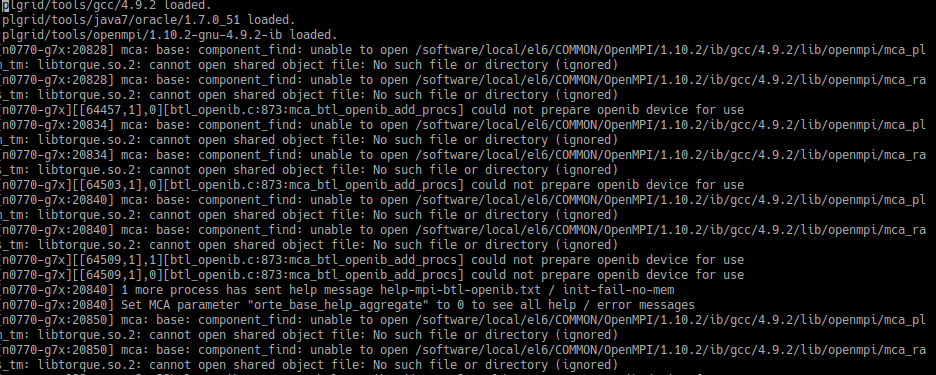
\includegraphics[scale=0.65]{pics/error_1.png}
\caption{Wynik zwrócony po uruchomieniu z --constraint="intel" oraz z i bez flagi --exclusive.}
\end{figure}

\begin{figure}[h]
\centering
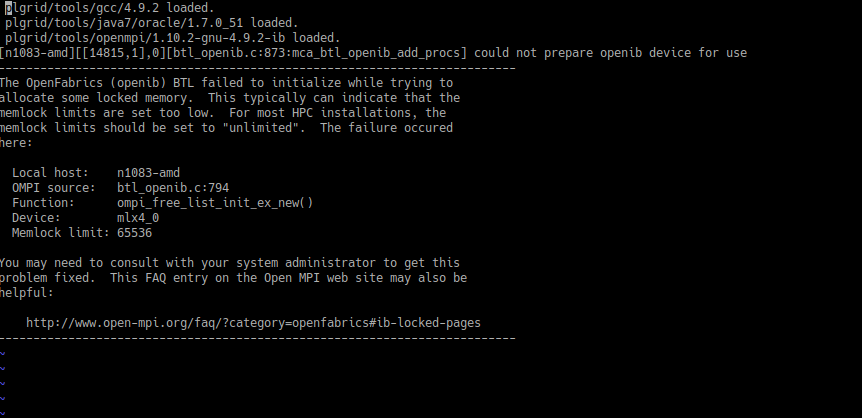
\includegraphics[scale=0.7]{pics/error_2.png}
\caption{Wynik zwrócony po uruchomieniu bez --constraint="intel" i bez --exclusive.}
\end{figure}

Każda część eksperymentu została powtórzona trzykrotnie dla uśrednienia wyników i wyeliminowania błędów grubych, które mogłyby wynikać z chwilowego przeciążenia architektury przez innego użytkownika. Trzykrotne wykonanie jest niewielką próbką i dla uzyskania bardziej wiarygodnych wyników należałoby powtórzyć próbę kilkaset razy, ale z uwagi na dzielenie zasobów nie podjęto takich kroków. Do wyciągnięcia wniosków z zadanego ćwiczenia kilkurotne, zgrubne uśrednienie jest wystarczające. 

Polecam do otwarcia Excela użyć wersji desktopowej, bo w takiej był przygotowany. Otwarcie w przeglądarce zmienia wygląd wykresów.

\chapter{Wykresy}
Do przedstawienia wyników zostały użyte wykresy liniowe, bez zazanaczenia punktów pomiaru aby nie zaciemniać wykresu. Dla zależności czasu wykonania od ilości procesorów umieszczono jednocześnie na wykresie wartości z wersji skalowane i nieskalowanej, dlatego że wartości mają podobne rzędy wielkości. Przy umieszczeniu osobno na dwóch wykresach: trzech trendów skalowanych i trzech nieskalowanych, czasy dla problemów małych i średnich wygladają jak płaskie kreski na poziomie 0 w porównaniu z problemem dużym. Nie dawało to wystarczającej informacji o kształcie wykresów, a informacja ta jest ważna, więc w przedstawieniu czasów przyjęto inną formę niż w pozostałych metrykach. Wykresy przyśpieszenia, efektywności i części sekwencyjnej są sporządzone według sugestii z instrukcji do ćwiczenia.

\begin{figure}[H]
\centering
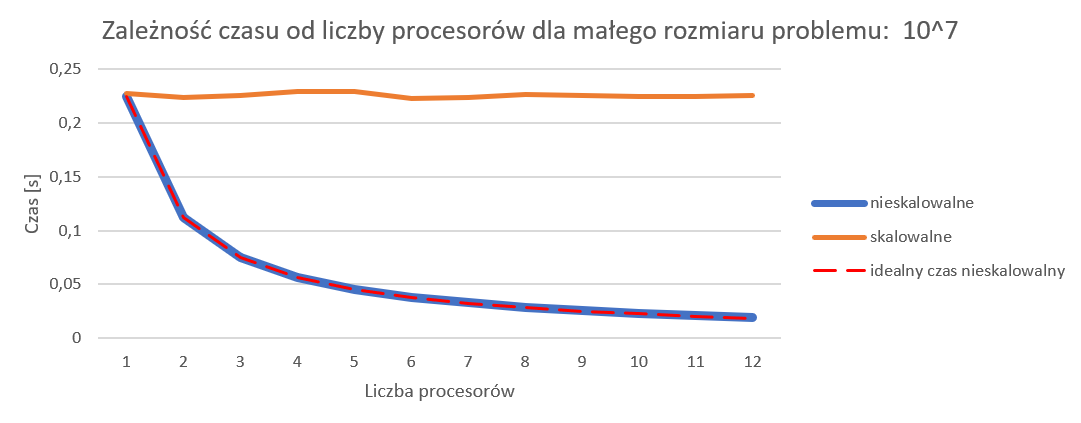
\includegraphics[scale=0.9]{pics/small.png}
\caption{Wykres czasu dla małego problemu.}
\end{figure}

\begin{figure}[H]
\centering
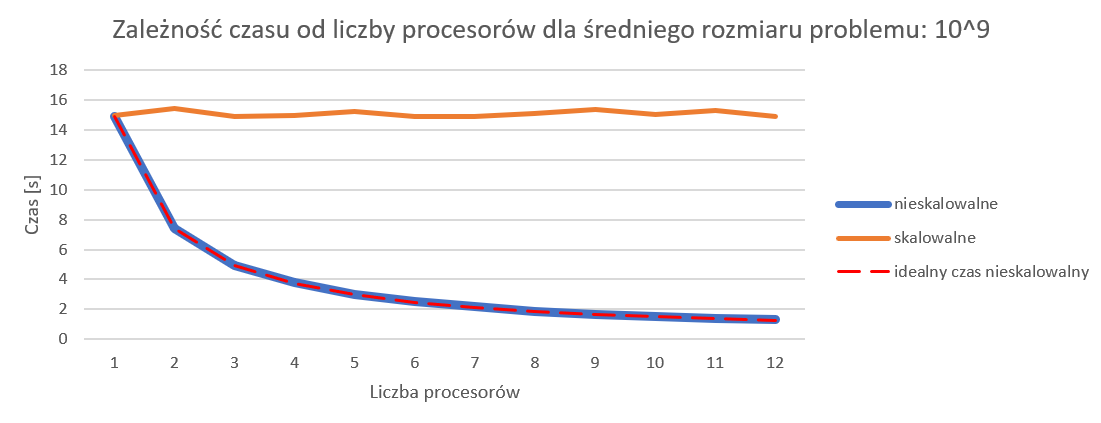
\includegraphics[scale=0.9]{pics/medium.png}
\caption{Wykres czasu dla średniego problemu.}
\end{figure}

\begin{figure}[H]
\centering
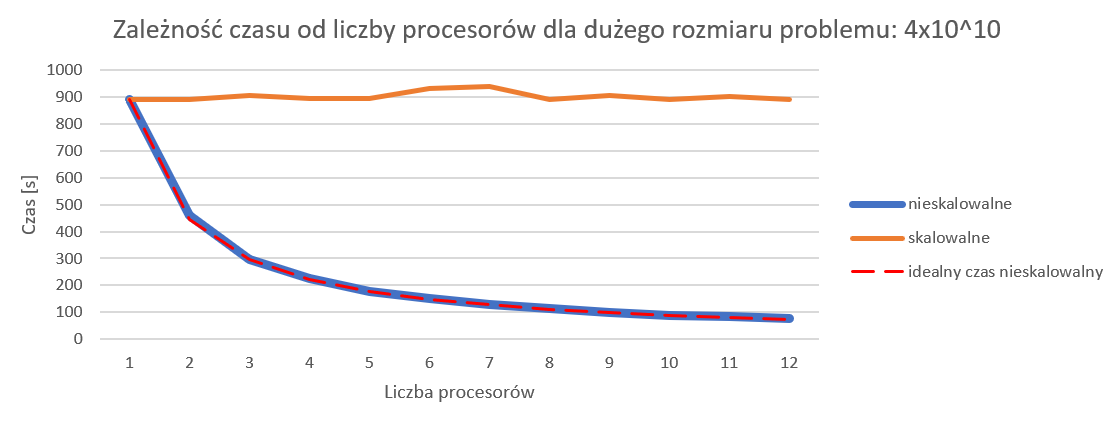
\includegraphics[scale=0.9]{pics/big.png}
\caption{Wykres czasu dla dużego problemu.}
\end{figure}

Jak można zauważyć wszystkie trzy wykresy są bardzo do siebie podobne. Główną różnicą jest skala na osi pionowej, wahająca się od części setnych sekundy po tysiąc sekund. 

Dla warsji ze skalowaniem idealną charakterystyką jest linia prosta. Biorąc pod uwagę małą skalę wykresu dla małych danych czas dla ćwiczenia skalowanego jest za każdym razem taki sam. Jest to tak mały problem, że "nie ma czasu" na zarejestrowanie różnic. Dla skalowania średniego wahania - zważając na skalę - są już większe. Widać fluktuacje wielkości, które jednak są na tyle losowe, że mieszczą się w granicach błędu statystycznego. Dla dużego problemu widać uskok na poziomie 6-7 procesorów. Jest to różnica rzędu 20-30 sekund, co jest znaczącym skokiem w porównaniu z poprzednio opisywanymi trendami. Według szczegółowych danych z Excela widać, że skok nie jest spowodowany podniesieniem wartości jednej próbki, lecz wszystkich trzech na raz. Uważam więc, że jest to cecha architektury, na której program został wykonany. Najwyraźniej któryś z procesorów , który został włączony do użycia na poziomie 6-7 jest inny niż wcześniej używane procesory - program wykonuje się na nim nieznacznie dłużej i przez to reszta musiała czekać, co wydłużyło sumaryczny czas pracy.

W wersji bez skalowania idealną charakterystykę uzyskano dzieląc czas referencyjny (wykonania programu na 1 procesorze) przez liczbę procesorów. Jak widać trend "idealny" pokrywa się dla każdego rozmiaru problemu z trendem nieskalowanym. Jedynie dla dużego problemu lekko podnosi się na poziomie dwóch procesorów - tylko jeden pomiar na 3 jest zgodny z idealnym wynikiem. Mogłoby to oznaczać tak jak poprzednio użycie innego procesora, jednak w tym przypadku może to być również błąd losowy, który zniknąłby po wykonaniu większej liczby pomiarów.
\section{Metryki skalowane}

\begin{figure}[H]
\centering
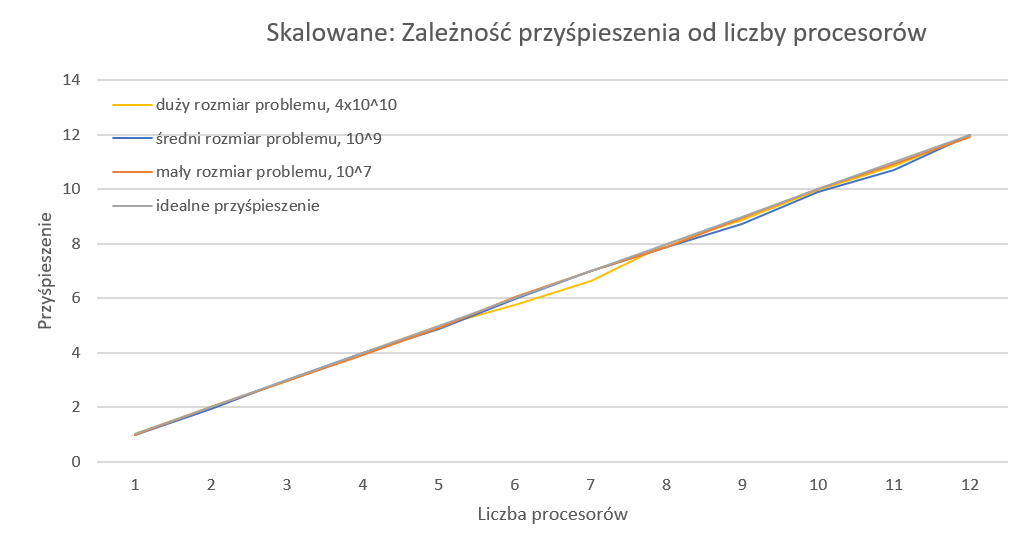
\includegraphics[scale=0.9]{pics/Sk_speedup.png}
\caption{Wykres przyśpieszenia dla małego problemu.}
\end{figure}

Linie prawie idealnie się pokrywają poza odchyleniem dla dużego problemu na poziomie 6-7 procesora. Jest to zrozumiałe, że wydłużony czas wykonania programu zmniejsza przyśpieszenie.

\begin{figure}[H]
\centering
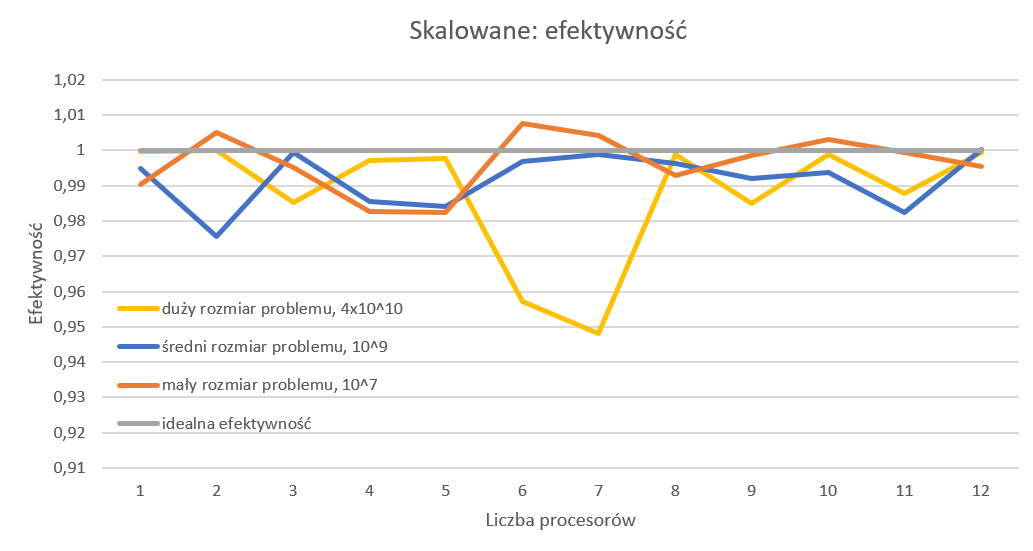
\includegraphics[scale=0.9]{pics/Sk_efekt.png}
\caption{Wykres efektywności dla średniego problemu.}
\end{figure}

\begin{figure}[H]
\centering
\includegraphics[scale=0.9]{pics/Sk_sekw.png}
\caption{Wykres udziału części sekwencyjnej dla dużego problemu.}
\end{figure}

Skok w czasie dla dużego problemu skalowalnego na poziomie 6-7 procesorów jest szczególnie widoczny tutaj - w metrykach efektywności i części sekwencyjnej. Efektywność widocznie spada, a udział części sekwencyjnej rośnie w tych obszarach. Poza tym dość dużym odchyleniem od normy charakteryzuje się trend średni dla części sekwencyjnej przy 2 procesorach. Nie ma to odzwierciedlenia w innych wykresach - pomiary dla p=2 i średniego rozmiaru nie odbiegają znacznie od reszty dla czasu, przyśpieszenia czy efektywności. Uważam, że jest to cecha tego rodzaju metryki - dla nawet małych błedów w liczniku wzoru przy małej liczbie procesorów błąd ten jest mnożony razy 2. Przy 3 procesorach błąd mnożymy już tylko razy 1,5 itd. Łatwo więc o duży skok spowodowany małym błędem pomiarowym właśnie szczególnie gdy procesorów jest mało. Tę teorię potwierdza też sam wykres - fluktuacje wygaszają się wraz ze wzrostem liczby procesorów.

Reszta wahań w tych wykresach jest marginalna i jest skutkiem małych odchyleń losowych, o których była mowa w omówieniu wykresu zależności czasu od liczby procesorów. Efektywność powyżej 100\% dla małego problemu nie jest objawem super liniowości (nie ma podstaw do jej uzyskania, typu eliminacja przepełnień cache), lecz błędów pomiaru dla małej próbki i małego rozmiaru problemu. Tego typu zjawiska nie obserwujemy już dla średniego i dużego problemu, bo wyniki dla dużych prób są wiarygodniejsze i mniej podatne na tego typu błędy.

\section{Metryki nieskalowane}

\begin{figure}[H]
\centering
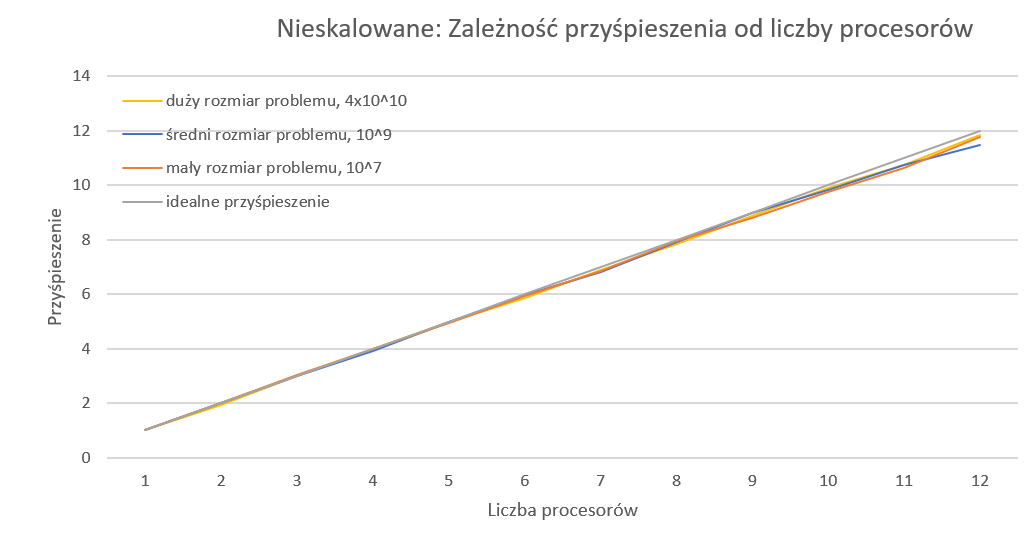
\includegraphics[scale=0.9]{pics/Ns_speedup.png}
\caption{Wykres przyśpieszenia dla małego problemu.}
\end{figure}

\begin{figure}[H]
\centering
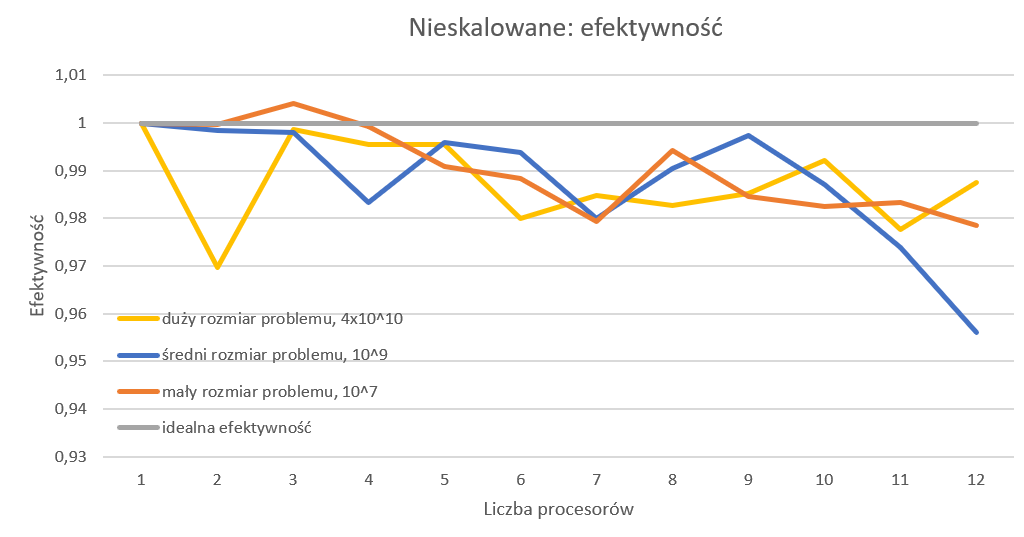
\includegraphics[scale=0.9]{pics/Ns_efekt.png}
\caption{Wykres efektywności dla średniego problemu.}
\end{figure}

\begin{figure}[H]
\centering
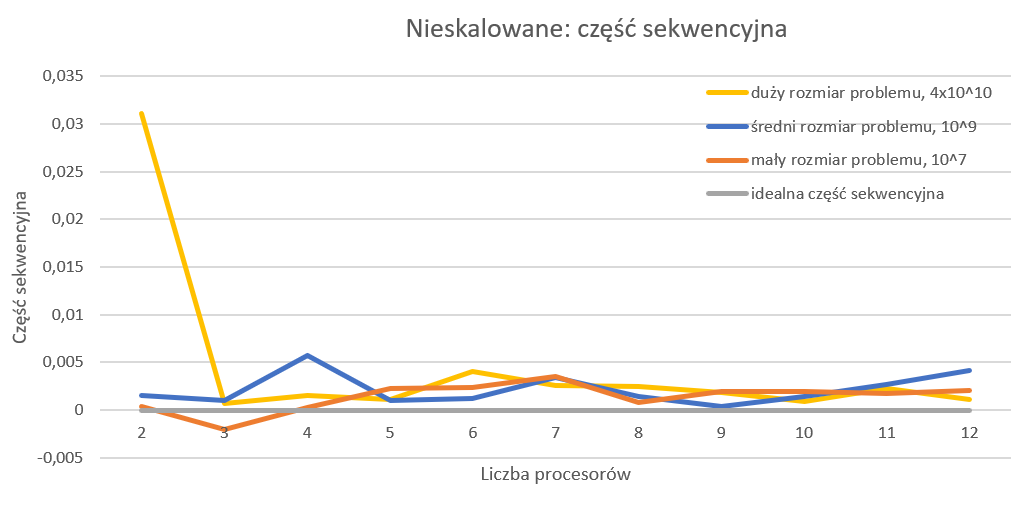
\includegraphics[scale=0.9]{pics/Ns_sekw.png}
\caption{Wykres udziału części sekwencyjnej dla dużego problemu.}
\end{figure}

Tak samo jak w przypadku skalowalnym można zauważyć efektywność ponad 100\% dla małego problemu. Wytłumaczenie jest takie samo. Podobnie jak dla wykresu skalowanego: dla części sekwencyjnej występuje pik przy małej liczbie procesorów.

\chapter{Użyte wzory}
Przyśpieszenie nieskalowane. T(1) - czas dla 1 procesora, T(p) - czas dla p procesorów.
\begin{equation}
s(p)=\frac{T(1)}{T(p)}
\end{equation}

Przyśpieszenie skalowane. T(1,1) - czas dla 1 procesora i skali k=1, T(p, k) - czas dla p procesorów i zadania przeskalowanego o skalę k.
\begin{equation}
s(p,k)=k \frac{T(1,1)}{T(p,k)}
\end{equation}

Efektywność (dla skalowanej bierzemy s(p,k) zamiast s(p) do wzoru):
\begin{equation}
E(p) = \frac{s(p)}{p}
\end{equation}

Część sekwencyjna (dla skalowanej bierzemy s(p,k) zamiast s(p) do wzoru):
\begin{equation}
f(p) = \frac{\frac{1}{s(p)} - \frac{1}{p}}{1 - \frac{1}{p}}
\end{equation}

\justifying

\end{document}